\documentclass[a4paper,12pt]{article}
%	options include 12pt or 11pt or 10pt
%	classes include article, report, book, letter

%% Always need these
\usepackage[utf8]{inputenc}
\usepackage[a4paper,pagebackref,hyperindex=true]{hyperref} % load hyperref before algorithm!!!!!!!
\usepackage{subfigure}
\usepackage{algorithm}
\usepackage{algorithmic}
\usepackage{amsmath}
\usepackage{fancyhdr}

%% Colored links in pdf
\usepackage{color}
\newcommand{\blue}{ \color{blue} }
\definecolor{linkcol}{rgb}{0,0,0.4}
\definecolor{citecol}{rgb}{0.5,0,0}

%% Bibliography text
% nicer backref links
\renewcommand*{\backref}[1]{}
\renewcommand*{\backrefalt}[4]{%
\ifcase #1 %
(Not cited.)%
\or
(Cited on page~#2.)%
\else
(Cited on pages~#2.)%
\fi}
\renewcommand*{\backrefsep}{, }
\renewcommand*{\backreftwosep}{ and~}
\renewcommand*{\backreflastsep}{ and~}

%% Language
\usepackage[ngerman,english]{babel}
\selectlanguage{ngerman}

%% Fonts
\usepackage[T1]{fontenc}
\usepackage{amsfonts} % need for mathbb
\usepackage[font=footnotesize,labelfont=bf]{caption} % small captions
%
% Latin Modern
%\usepackage{lmodern}
%
% Computer Concrete
%\usepackage{concmath}
%
% Utopia Regular with Math Design
%\usepackage[adobe-utopia]{mathdesign}
%
% Charter
\usepackage{charter}

%% Code
\usepackage{listings}
\lstset{ %
  language=C++, % choose the language of the code
  basicstyle=\small\ttfamily, % the size of the fonts that are used for the code
  numbers=left, % where to put the line-numbers
  numberstyle=\small\ttfamily\color[rgb]{0.6,0.6,0.6}, % the size of the fonts that are used for the line-numbers
  stepnumber=1, % the step between two line-numbers. If it's 1 each line
  xleftmargin=4mm,
  % will be numbered
  numbersep=5pt, % how far the line-numbers are from the code
  backgroundcolor=\color{white}, % choose the background color. You must add \usepackage{color}
  showspaces=false, % show spaces adding particular underscores
  showstringspaces=false, % underline spaces within strings
  showtabs=false, % show tabs within strings adding particular underscores
%  frame=l, % adds a frame around the code
  frame=single,
  tabsize=2, % sets default tabsize to 2 spaces
  breaklines=true, % sets automatic line breaking
  breakatwhitespace=false, % sets if automatic breaks should only happen at whitespace
  % also try caption instead of title
  escapeinside={@}{@}, % if you want to add a comment within your code
  morekeywords={*,...}, % if you want to add more keywords to the set
  keywordstyle=\color[rgb]{0,0,1},
  commentstyle=\color[rgb]{0.133,0.545,0.133}\textit,
  stringstyle=\color[rgb]{0.627,0.126,0.941},
}

%% Customizations
\newenvironment{packed_item}{
\vspace{-2mm}
\begin{itemize}
  \setlength{\itemsep}{1.5pt}
  \setlength{\parskip}{0pt}
  \setlength{\parsep}{0pt}
}{\vspace{-2mm}\end{itemize}}

\newenvironment{abstr}{%
\vfill\small%
\begin{center}%
{\bfseries \abstractname}%
\end{center}%
\quotation}%
{\vfill}%

\newenvironment{todocontent}{%
\begin{outline}
\color[rgb]{0.6,0.6,0.6}
}{%
\end{outline}
}% End environment

% Provide the \*matter commands in non-book classes
\providecommand{\frontmatter}{%
\clearpage%
\pagenumbering{roman}%
\setcounter{page}{1}}%

\providecommand{\mainmatter}{%
\clearpage%
\pagenumbering{arabic}%
\setcounter{page}{1}%
\pagestyle{fancy}%
\fancyhf{}%
\fancyhead[L]{\leftmark}%
\fancyhead[R]{\thepage}%
}%

\providecommand{\backmatter}{%
\clearpage%
\pagenumbering{arabic}%
\setcounter{page}{1}}%

% Paragraph Intendation
\setlength{\parindent}{0pt}
\setlength{\parskip}{2ex}

%% todonotes. gives command \todo{do this thing}
\usepackage{todonotes}

%% Outlines
\usepackage{outlines}

%% Include macros
%% general vector style (bold or with arrow)
\newcommand{\ve}[1]{
    \mathbf{#1}
    %\vec{#1}
}

%% Specific to this thesis
\newcommand{\eps}{\varepsilon}

%% common shortcuts
\providecommand{\argmin}{\operatorname*{argmin}} % operatorname makes _{..} appear centered
\providecommand{\argmax}{\operatorname*{argmax}} % operatorname makes _{..} appear centered
\newcommand{\dd}[1]{\,\mathrm{d}#1} % integration: \int f(x) \dd{x}
\newcommand{\EE}{\mathbb{E}}        % expectation value
\newcommand{\RR}{\mathbb{R}}        % set of real numbers
\newcommand{\CC}{\mathbb{C}}        % set of complex numbers
\newcommand{\NN}{\mathbb{N}}        % set of natural numbers
\newcommand{\OO}{\mathcal{O}}       % big O notation (asymptotic complexity)
\newcommand{\TT}{\mathbb{T}}        % time interval

%% Vectors (lowercase letters)
\renewcommand{\a}{\ve{a}}
\renewcommand{\b}{\ve{b}}
\renewcommand{\c}{\ve{c}}
\renewcommand{\d}{\ve{d}}
\newcommand{\e}{\ve{e}}
\newcommand{\f}{\ve{f}}
\newcommand{\g}{\ve{g}}
\newcommand{\h}{\ve{h}}
\renewcommand{\i}{\ve{i}}
\renewcommand{\j}{\ve{j}}
\renewcommand{\k}{\ve{k}}
\renewcommand{\l}{\ve{l}}
\newcommand{\m}{\ve{m}}
\newcommand{\n}{\ve{n}}
\renewcommand{\o}{\ve{o}}
\newcommand{\p}{\ve{p}}
\newcommand{\q}{\ve{q}}
\renewcommand{\r}{\ve{r}}
\newcommand{\s}{\ve{s}}
\renewcommand{\t}{\ve{t}}
\renewcommand{\u}{\ve{u}}
\renewcommand{\v}{\ve{v}}
\newcommand{\w}{\ve{w}}
\newcommand{\x}{\ve{x}}
\newcommand{\y}{\ve{y}}
\newcommand{\z}{\ve{z}}

%% Matrices (uppercase letters)
\newcommand{\A}{\ve{A}}
\newcommand{\B}{\ve{B}}
\newcommand{\C}{\ve{C}}
\newcommand{\D}{\ve{D}}
\newcommand{\E}{\ve{E}}
\newcommand{\F}{\ve{F}}
\newcommand{\G}{\ve{G}}
\renewcommand{\H}{\ve{H}}
\newcommand{\I}{\ve{I}}
\newcommand{\J}{\ve{J}}
\newcommand{\K}{\ve{K}}
\renewcommand{\L}{\ve{L}}
\newcommand{\M}{\ve{M}}
\newcommand{\N}{\ve{N}}
\renewcommand{\O}{\ve{O}}
\renewcommand{\P}{\ve{P}}
\newcommand{\Q}{\ve{Q}}
\newcommand{\R}{\ve{R}}
\renewcommand{\S}{\ve{S}}
\newcommand{\T}{\ve{T}}
\newcommand{\U}{\ve{U}}
\newcommand{\V}{\ve{V}}
\newcommand{\W}{\ve{W}}
\newcommand{\X}{\ve{X}}
\newcommand{\Y}{\ve{Y}}
\newcommand{\Z}{\ve{Z}}

% Macro for 'List of Symbols', 'List of Notations' etc...
\def\listofsymbols{\input{symbols} \clearpage}
\def\addsymbol #1: #2#3{$#1$ \> \parbox{115mm}{#2 \dotfill \pageref{#3}}\\}
\def\newnot#1{\label{#1}}

\newcommand*{\nom}[3][\empty]{%%% \empty: Standardwert des optionalen Parameters
  \ifthenelse{\equal{#1}{\empty}}%
    {#2\nomenclature{#2}{#3}}%
    {#2\nomenclature[#1]{#2}{#3}}%
}



\hypersetup
{
bookmarksopen=true,
pdftitle=Example Thesis,
pdfauthor=Author Name,
pdfsubject=ShortTitle, %subject of the document
%pdftoolbar=false, % toolbar hidden
pdfmenubar=true, %menubar shown
pdfhighlight=/O, %effect of clicking on a link
colorlinks=true, %couleurs sur les liens hypertextes
pdfpagemode=None, %aucun mode de page
pdfpagelayout=SinglePage, %ouverture en simple page
pdffitwindow=true, %pages ouvertes entierement dans toute la fenetre
linkcolor=linkcol, %couleur des liens hypertextes internes
citecolor=citecol, %couleur des liens pour les citations
urlcolor=linkcol %couleur des liens pour les url
}

\usepackage{draftwatermark} %% DRAFT watermark

%
%% Begin the document
%
\begin{document}
\frontmatter

\begin{titlepage}
\begin{center}
    \vspace*{1cm}
    %\title{Implementierung rheologisch komplexer Materialmodelle in OpenFOAM}
    {\huge \bfseries Title\\}
    \vspace{2cm}
    {\large 
        Author\\
	~\\
	Studiengang Rechnergestützte Wissenschaften Master\\
	\vspace{3.5cm}
	Masterarbeit HS 2012\\
	~\\
	Institut für Fluiddynamik\\
	ETH Zürich\\
    }

\vspace{\stretch{1}}



{\large
	Betreuer: \ldots\\[\baselineskip]
	Professor: \ldots
}
\end{center}

\vspace*{2cm}

\end{titlepage}


\thispagestyle{empty}
\selectlanguage{ngerman}
\begin{abstr}
Deutsche Zusammenfassung
\end{abstr}

\selectlanguage{english}

\begin{abstr}
English abstract
\end{abstr}


\newpage
\tableofcontents
\newpage
%\section*{List of Symbols\hfill}% \addcontentsline{toc}{chapter}{List of Symbols}
%\listofsymbols
\renewcommand{\nomname}{List of Symbols}
\printnomenclature[3em]

% Actual thesis
\mainmatter
\section{Section}
\label{section}

\subsection{Subsection}
\label{subsection}

\subsubsection{Notation, Todo and Citation}
\label{notation}
There is a stopping region $\Gamma_S$ \newnot{symbol:GammaS} of width $\delta>0$. \newnot{symbol:delta}
\cite{Muller}
\todo{add a picture here}

\subsubsection{Code}
Code:
\begin{lstlisting}
void Scheduler<SchedulingAlgorithm, spacedimV>::schedule(){
// Get number of available cores
int nCores = MPI::COMM_WORLD.Get_size();

// Create instance of scheduling algorithm
SchedulingAlgorithm schedulAlgo;
// And call its scheduling method
schedulAlgo.schedule( 
        // number of available cores
        nCores,
        // List with problem weights, problem i has a computational complexity of problemSizes[i]
        problemSizes,
        // List of lists to be filled with the scheduling, problem i is calculated on all cores contained in the list problemToCore[i]
        problemToCore
);

}
\end{lstlisting}

\subsubsection{Outline}
Example of outline:
\begin{outline}
    \1 First level
        \2 Second level
            \3 Third level
        \2[+] Second level with custom symbol
    \1 Again first level
        \2[] Second level without symbol
\end{outline}
\begin{outline}[enumerate]
    \1 Numerated outline
        \2 Second level
            \3 Third level
\end{outline}

\subsubsection{Pictures}
Example of subfloats with separate labeling:
Figure~\ref{fig:strongscalingfull} shows the timing \subref{fig:sub:strongscalingfulltiming} and the efficiency plot \ref{fig:sub:strongscalingfullefficiency} for the RTE solver with the full tensor solution method.
\begin{figure}[h]
    \centering
    \subfloat[Timings]{
        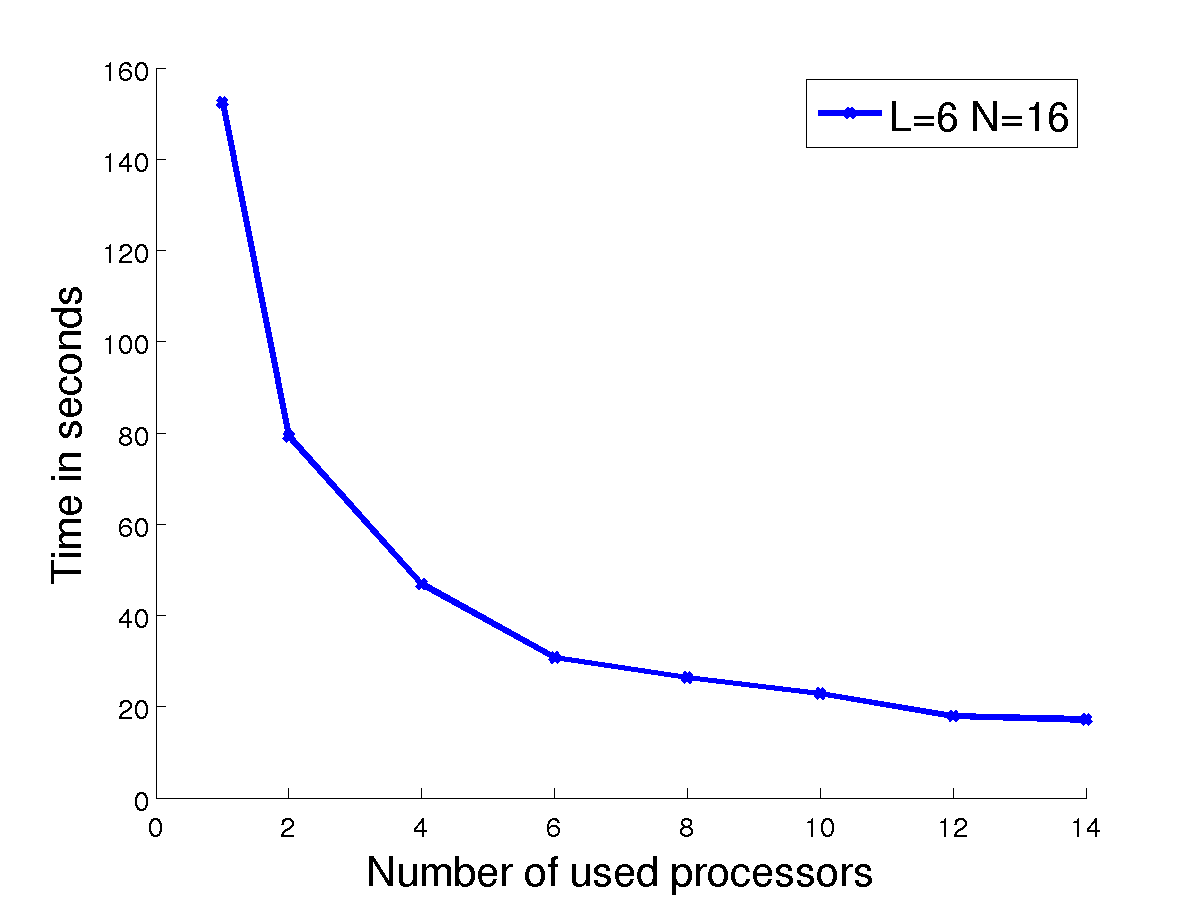
\includegraphics[height=40mm]{figures/strongscalingfulltiming.png}
        \label{fig:sub:strongscalingfulltiming}
    }
    \subfloat[Efficiency]{
        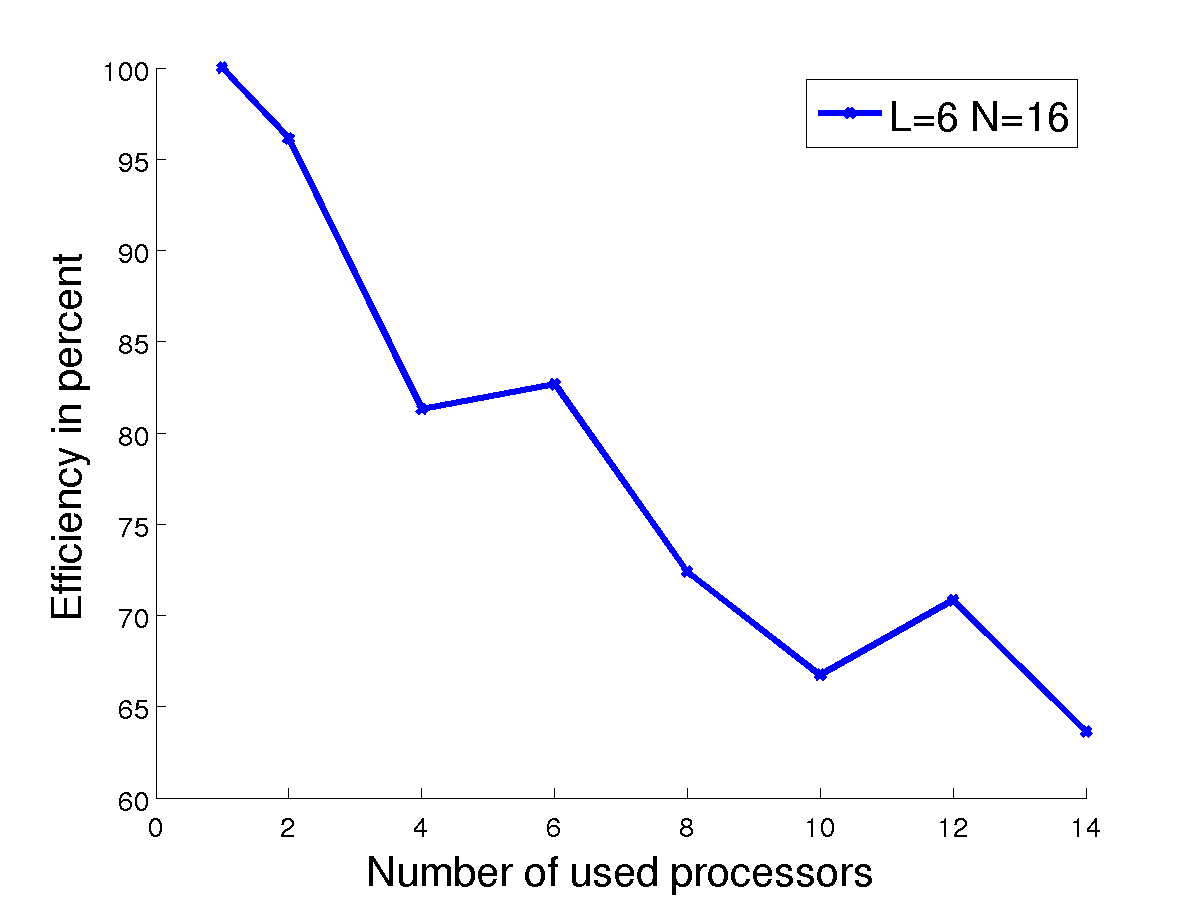
\includegraphics[height=40mm]{figures/strongscalingfullefficiency.png}
        \label{fig:sub:strongscalingfullefficiency}
    }
    \caption{Strong scaling of the RTE solver with the full tensor method. On the left the timing results are shown, on the right the according efficiency numbers are plotted.}
    \label{fig:strongscalingfull}
\end{figure}

\subsubsection{todocontent}
The todocontent environment is a customizable outline environment to help making the outline of a text.
\begin{todocontent}
    \1 This chapter should contain information about cows
    \1 And not to forget milk!
\end{todocontent}


\backmatter
%%% Bibliography
\bibliographystyle{ThesisStyleWithEtAl}
%\bibliographystyle{ThesisStyle}
%\bibliographystyle{plain}
\bibliography{sources}

\end{document}
